%----------------------------------------------------------------------------
\chapter{Választott technológiák}
%----------------------------------------------------------------------------

Annek a fejezetnek a keretein belül a felhasznált technológiák kiválasztásának szempontjait szeretném bemutatni. 
Elöszőr a frontend technológiát választottam ki úgyanis az alkalmazásnak ez a része a bonyolultabb a raktár térképek kezelése miatt.
%----------------------------------------------------------------------------

\section{Frontend}

A piacon jelenleg 3 meghatározó keretrendszer/könyvtár érhető el, melyek segítségével webes alkalmazások felhasználói felületét készíthetjük el.

Ezek az Angular, a React és a Vue. 
Bár mind a három keretrendszer célja ugyan az mégis nagy eltéréseket tapasztalhatunk a kódbázisban, felépítésben és a fejlesztúk filozofiájában.
%----------------------------------------------------------------------------

\subsection{Angular}

Az Angular a Google által 2010-ben elinditott és a mai napig általuk karbantartott keretrendszer.
Filozofiája az, hogy egy általános felhasználásra felkészített alapot ad. 
Tartalmazza a formok validációját, az állapot kezelést, a routing-ot és a felhasználói input-ok kezelését és ezen kivül még rengeteg más olyan dolgot is, ami hasznos lehet egy webalkalmazás fejlesztéséhez.
%----------------------------------------------------------------------------

\subsection{React}

Az Angular-hoz hasonlóan a React mögött is egy nagy cég áll.
A Facebook 2013 óta fejleszti és tartja karban a keretrendszert.
Az Angularral szemben a React, filozofiája szerint csak egy könnyű sulyú keretet ad. 
Emiatt talán nem is nevezhetjük keretrendszernek, sokkal inkább csak egy könyvtár. 
Azonban ennek és a fejlesztők által implementált virtuális DOM-nak köszönhetően sokkal jobb sebesség érhető el vele.
Természetesen az, hogy csak egy keretet ad nem okoz semmilyen hátrányt.
Ugyanis rengeteg hivatalos csomag érhető el hozzá, melyek megvalósítják az Angular által is nyujtott megoldásokat.
%----------------------------------------------------------------------------

\subsection{Vue}
A három keretrendszer közül a legújabb és legkevesebb fejlesztői erőforrással rendelkező opció.
A fejlesztését 2014-ben kezdte a Google egyik korábbi mérnöke, aki a mai napig szerves részét képezi a projektnek.
Filozofiáját tekintve a korábban tárgyalt két rendszer között helyezhető el. Többet tartalmaz, mint a React de korán sem annyit, mint az Angular. Itt is találkozhatunk a virtuális DOM-mal melynek köszönhetően nagyon gyors a működése.
Az összehasonlított keretrendszerek közül ezzel a legkönnyeb elkezdeni a fejlesztést, egy egyszerű alkalmazás elkészítése nem igényel sok ismeretet a HTML, CSS és JavaScript-en kívül. Természetesen komplex alkalmazásokat is készíthetünk vele, ipari környezetben is remekül megállja a helyét. 
%----------------------------------------------------------------------------

\subsection{Trendek}
A döntés meghozása elött végeztem egy kisebb kutatást a napjainkban tapasztalható trendekről. Ehhez a Google Trends és az NPM Trends szolgáltatásait vettem igénybe. Előbbi segitségével a Google keresések számát tudjuk összehasonlítani, míg utóbbival az NPM csomagkezelő oldalról történő letöltések számát.

\begin{figure}[!ht]
  \centering
  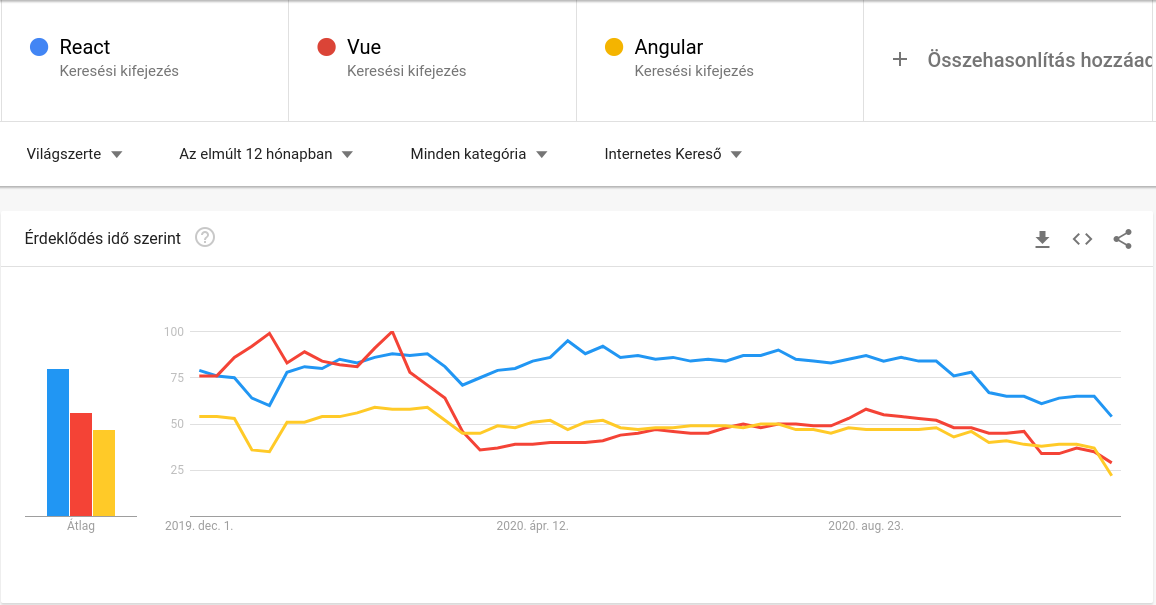
\includegraphics[width=150mm, keepaspectratio]{figures/google_trends.png}
  \caption{Google Trends - keresések összehasonlítása.}
  \label{fig:GoogleTrends}
\end{figure}

A Google keresések alapján a korábbi években az Angular egyértelműen uralta a piacot, azonban a vezető szerepet mára már átvette tőle a React, ahogy az a grafikonon (\refstruc{fig:GoogleTrends}) is látszik.

\begin{figure}[!ht]
  \centering
  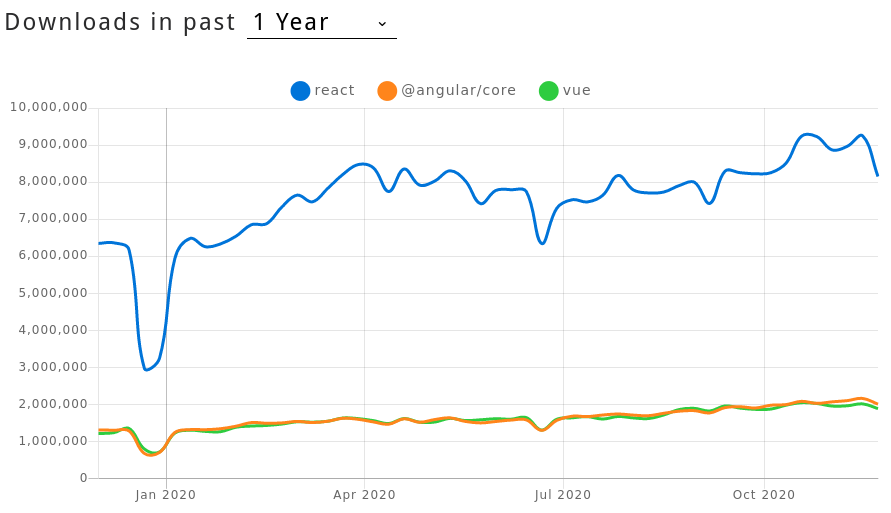
\includegraphics[width=150mm, keepaspectratio]{figures/npm_trends.png}
  \caption{NPM Trends - letöltések összehasonlítása.}
  \label{fig:NPMTrends}
\end{figure}

A Google keresések nem mutattak szignifikáns különbséget, azonban az NPM letöltések számában már jelentős eltéréseket tapasztalhatunk. A grafikonról (\refstruc{fig:NPMTrends}) könnyedén leolvasható, hogy több, mint 4-szer annyi a letöltések száma a React esetén, mint a másik 2 keretrendszernél.
%----------------------------------------------------------------------------

\subsection{Konkluzió}
A fent felsoroltakat alapul véve végül a React-re esett a választásom. A virtuális DOM és az aktív fejlesztői közösség hatalmas elönyt jelent a fejlesztés során. A döntést segítette, hogy ezzel a keretrendszerrel már volt szerencsém dolgozni és pozitív élmény volt.
%----------------------------------------------------------------------------

\section{Backend}

A kliens oldali technológia kiválasztása után a szerver oldali keretrendszer kiválasztására keürlt sor.
Itt sokkal több népszerű és az iparban is használt keretrendszer érhető el. Ilyen például a DotNet, a Spring, a Laravel, a Ruby on Rails, a Django és rengeteg rajtuk kívűl. Ezek összehasonlítása nagyon nehéz, így megpróbáltam egyszerűsíteni a folyamatot. Az elsődleges szempont a kiválasztás során az, hogy a választott frontend technológiával a legegyszerűbben és a legjobban tudjon egyött működni. Természetesen a felsorolt és a nem felsorolt keretrendszerek is működnek React-tel probléma nélkül. Azonban egy kiemelkedik közülük azáltal, hogy a programozási nyelv azonos frontend és backend oldalon is. Ez a NodeJS. Az azonos programozási nyelv felveti a kódmegosztás lehetőségét is a két komponens között. 
%----------------------------------------------------------------------------

\subsection{NodeJS}
A NodeJS története több, mint 11 éve indult Ryan Dahl keze által. A projekt a Google által fejlesztet V8 JavaScript motor segítségével teszi lehetővé JavaScript futtatását web böngészőn kívül, így lehetővé téve a nyelv felhasználását backend oldalon is. A NodeJS gyors ütemben fejlödött, 2011-ben már a Microsoft is kivette a részét a fejlesztésből napjainkra pedig az egyik legnépszerűbb technológia webes környezetben.
%----------------------------------------------------------------------------

\section{Kommunikációs megoldások}

A frontend és a backend technológiák kiválasztása után a következő lépés a köztük történő kommunikáció mikéntjének eldöntése volt.
Itt szerencsémre sokkal kevesebb opció közül kellett választanom. Napjainkban két fő irányvonal figyelhető meg. Ezek a REST API és a GraphQL.
%----------------------------------------------------------------------------

\subsection{REST API}
A REST feloldása REpresentational State Transfer, ami magyarra fordítva Reprezentatív Állapot Átvitel. Ez - ahogy a nevéből is következtetni lehet - probálja kifejező módon átvinni az adatot a kliens és a server alkalmazások között.
Ezt úgy valósítja meg, hogy ajánlást tesz a végpontok nevére és típusára rendeltetésük szerint.

\begin{table}[ht]
	\footnotesize
	\centering
	\begin{tabular}{ l c c l }
		\toprule
		Művelet angolul & Művelet magyarul & HTTP üzenet típusa & Végpont \\
		\midrule
		Create & Létrehozás & POST & /users \\
		Read & Megtekintés & GET & /users/:id \\
		Update & Módosítás  & POST & /users/:id \\
		Delete & Törlés  &  DELETE & /users/:id \\
		List & Listázás  & GET & /users \\
		\bottomrule
	\end{tabular}
	\caption{Példa egy entitáson végezhető müveletekre a REST API elvei szerint}
	\label{tab:RESTTable}
\end{table}
%----------------------------------------------------------------------------

\subsection{GraphQL}

A graphQL egy lekérdező nyelv, amely a jelenleg elterjedt REST API-s megoldásokat próbálja leváltani/kiegészíteni. A megszokott REST API-val ellentétben GraphQL-nél csak egyetlen egy végpont létezik, valamint csak POST típusú HTTP kéréseket használunk. 

Az összes kérést erre a végpontra küldjük a megfelelő tartalommal, melyet a POST kérés törzsében (body) helyezünk el.

A bevett REST API-s megoldással szembeni hatalmas előnye, hogy mindig azt kapjuk amit kérünk. A POST kérés törzsében elhelyezett GraphQL operation pontosan meghatározza, hogy milyen entitások milyen tulajdonságait szeretnénk visszakapni. Ez a GraphQL operation nagyon hasonlít a JSON formátumra, azonban egy-két dologban eltér attól. Lehetőségünk van több entitásból is adatot lekérni egyetlen kéréssel, így csökkentve a HTTP üzenetek számát.

A kéréseket minden esetben egy (vagy több) úgynevezett resolver szolgálja ki nekünk. 
A resolverekből 3 fő típust különböztetünk meg Query, Mutation és Subscription.

\subsubsection{Query}
Adatok lekérésére szolgál
  
\subsubsection{Mutation}
Ahogy a nevéből is következtethetünk rá főként adatok módosítására és létrehozására szolgál
  

\subsubsection{Subscription}
A standard GraphQL implementáció tartalmazza a websocket kommunikációt is. A subscription-ök segítségével lehetősége van a kliensnek feliratkozni bizonyos eseményekre, melyek bekövetkeztéről azonnal értesül socket kapcsolaton keresztül.
%----------------------------------------------------------------------------

\subsection{Konkluzió}
A fent leírt szempontokat figyelembe véve a végső választásomat a GraphQL mellett tettem le.
Tanulmányaim során rengetegszer találkoztam REST API-t használó vagy annak megvalósításák követelő feladattal, így ezen opció választása esetén nem mélyítettem volna el a tudásomat egy kevésbé ismert, azonban mégis remek technológiában.
%----------------------------------------------------------------------------

\section{Adatbázis}
Az alkalmazás nem rendelkezik olyan követelménnyel, amely komoly adatbázis műveletet igényel.
Ezért a választás szempont elsődlegesen az volt, hogy a már kiválasztott technológiákkal egyűtt a lehető legkényelmesebb és legjobb fejlesztési élményt nyújtsa. Ennek követelménye az volt, hogy adatbázisok helyett ORM rendszerek összehasonlítását kezdtem el.
Az ORM egy absztrakciós réteget helyez az adatbázis és az alkalmazás közé, így elfedve a lekérdező nyelvet, ez nagyobb biztonságot és gyorsabb fejlesztést eredményez.

Az ORM-ek többsége rengeteg dologban hasonlít, így az összehasonlítás során leginkább a különbségekre fókuszálok.
%----------------------------------------------------------------------------

\subsection{Sequelize}
Több, mint 7 éve elérhető ORM rendszer, az ötös verziótól beépített TypeScript támogatással érkezik.
A sequelize-cli segítségével generálhatunk modelleket és migrációkat is.
%----------------------------------------------------------------------------

\subsection{TypeORM}
Fejlesztése 5 éve kezdödött, azonban a mai napig sem érte el az 1.0-ás verziót.
Beépített TypeScript támogatással rendelkezik és a Sequelize-hoz hasonlóan generálhatunk modelleket és migrációkat.
%----------------------------------------------------------------------------


\subsection{Mongoose}
A Mongoose ORM a mongoDB kezeléséhez több, mint 10 évvel ezelőtt létrehozott csomag. 
Mivel a mongoDB egy document alapú NoSQL adatbáizs, így még fontosabb az adatok validációja.
A mongoose séma természetesen kezeli ezt, azonban a migrációk meglévő adatok esetén problémás és sok hibalehetőséget rejt.
A TypeScript támogatás megoldható de szintén körülményes.
%----------------------------------------------------------------------------

\subsection{Prisma}
2020 júniusában jelentették be a 2.0-ás verziót, amely az 1.0 alapoktól újraírt változata.
Teljes körű TypeScript támogatás érkezik és rengeteg extra funkcióval.
A migrációs generálása automatikus, így a séma módosítása után automatikus generálható bármilyen fejlesztői beavatkozás nélkül.
Természetesen ha adatmigráció is szükséges azt nekünk kell kezelnünk.
A Prisma egy beépített Studio nevű grafikus interface-szel érkezik, így teljes grafikus hozzáférést kapunk az adatbázishoz bármilyen külső megoldás nélkül.

%----------------------------------------------------------------------------

\subsection{Konkluzió}
Habár a trendek (\refstruc{fig:ORMTrends}) alapján a Prisma jócskán el van maradva népszerűségben az összehasonlításban részt vett többi ORM-től mégis erre esett a választásom.
A korábban felsorolt elönyök és a növekvő népszerűség miatt úgy érzem, hogy a lemaradása egyedül az újdonságának köszönhető.

Tekintve, hogy fejlesztése még mindig egy korai stádiumban van az adatbázis kezelők listája szükös.
A fejlesztés kezdetekor csak PostgreSQL, MySQL és SQLite volt támogatott, utobbi kisebb hiányoságokkal.
A dolgozat írása közben bejelentették a MSSQL támogatást is. 
A választáskor a MySQL és PostgreSQL között kellett döntenem.
Az adatbázisom bonyolultsága nem lesz túl nagy, így személyes preferencia alapján a PostgreSQL mellett döntöttem.
%----------------------------------------------------------------------------

\begin{figure}[!ht]
  \centering
  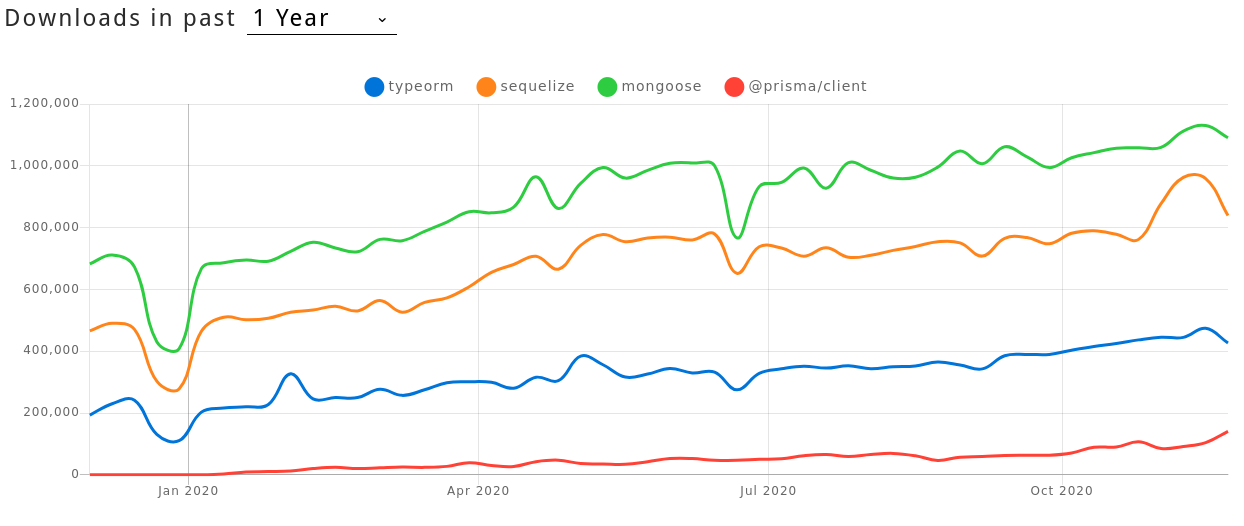
\includegraphics[width=150mm, keepaspectratio]{figures/orm_npm_trends.png}
  \caption{NPM Trends - ORM-ek letöltésének összehasonlítása.}
  \label{fig:ORMTrends}
\end{figure}

%----------------------------------------------------------------------------
\section{Közös technológiák}
%----------------------------------------------------------------------------
Ahogy azt a korábbi fejezetben is említettem a NodeJS-nek hála a backend és a frontend oldali alkalmazás azonos nyelvet használ, a JavaScript-et.
A JavaScript egyik nagy hátránya az, hogy gyengén típusos nyelv (természetesen ezt bizonyos esetekben tekinthetjük elönynek is). Ennek a megoldására JavaScript helyett TypeScript-et használtam az alkalmazás megvalósításához.

%----------------------------------------------------------------------------
\subsection{TypeScript}
%----------------------------------------------------------------------------

A TypeScript egy - a Microsoft által fejlesztett - nyílt forráskódú nyelv, amely JavaScript-et egészíti ki statikus típus definíciókkal. Mondhatjuk, hogy a JavaScript egy superset-je.

A típusok segítségével hamarabb észrevehetjük a hibákat az alkalmazásunkban. Azonban fontos megjegyezni, hogy a típusok definiálása opcionális, ezért TypeScript mellett érdemes valamilyen linter-t használni, amely figyelmezteti a programozót ha elmulasztja a típusdefiníciók használatát. 
Minden érvényes JavaScript kód egy érvényes TypeScript kód is, ez részben az elhagyható típusdefiníciók miatt igaz.

Annak érdekében, hogy probléma nélkül futtathassuk a TypeScript kódunkat a böngészőkben minden kódot JavaScript-re transzformálunk. Erre több megoldás is létezik, ilyen például a Babel vagy a TypeScript complier.

A NodeJS-nek köszönhetően használhatjuk backend oldali nyelvként is, így a frontend és a backend közös nyelvet használhat, amely akár a kódmegosztás lehetőségét is felveti.
